\documentclass{bioinfo}
\copyrightyear{2012}
\pubyear{2012}
\application

\usepackage{xspace}
\newcommand{\dsk}{DSK\xspace}
\newcommand{\jelly}{Jellyfish\xspace}
\newcommand{\bfc}{BFCounter\xspace}
\renewcommand{\thefootnote}{\fnsymbol{footnote}}

\usepackage{algorithm}
\usepackage[noend]{algorithmic} %remove end if, end for

\begin{document}
\firstpage{1}

\title[short title]{\dsk: $k$-mer counting with very low memory usage}
\author[G. Rizk \textit{et~al}]{Guillaume Rizk\,$^{1,*}$, Dominique Lavenier\,$^{2}$ and Rayan Chikhi\,$^2$%\footnote{to whom correspondence should be addressed}
}
\address{$^{1}$Algorizk, 75013 Paris, France\\
$^{2}$ENS Cachan Brittany / IRISA, Campus de Beaulieu, 35700 Rennes, France}

\history{Received on XXXXX; revised on XXXXX; accepted on XXXXX}

\editor{Associate Editor: XXXXXXX}

\maketitle

\begin{abstract}

\section{Summary:}
Counting all the $k$-mers (substrings of length $k$) in DNA/RNA sequencing reads is the preliminary step of many bioinformatics applications. However, state of the art $k$-mer counting methods require that a large data structure resides in memory. Such structure typically grows with the number of distinct $k$-mers to count. 

We present a new streaming algorithm for $k$-mer counting, called \dsk (\textbf{d}isk \textbf{s}treaming of $\mathbf{k}$-mers), which only requires a fixed, user-defined amount of memory and disk space.
This approach realizes a memory, time and disk trade-off. The multi-set of all $k$-mers present in the reads is partitioned and partitions are saved to disk. Then, each partition is separately loaded in memory in a temporary hash table. The $k$-mer counts are returned by traversing each hash table. Low-abundance $k$-mers are optionally filtered.

\dsk is the first approach that is able to count all the $27$-mers of a human genome dataset using only 4.0 GB of memory and moderate disk space (160 GB), in 17.9 hours. \dsk can replace a popular $k$-mer counting software (Jellyfish) on small-memory servers.
\section{Availability:}
%The \dsk software is available at\\
 \href{http://minia.genouest.org}{http://minia.genouest.org/dsk}

\section{Contact:} \href{guillaume.rizk@gmail.com}{rayan.chikhi@ens-cachan.org}
\end{abstract}
\section{Introduction}
Determining the abundance of each distinct $k$-mer in a set of sequencing reads is a conceptually simple yet fundamental task. It is used in many bioinformatics applications related to sequencing, e.g. genome and transcriptome assembly, variants detection and read error correction. For \emph{de novo} assembly, one is often interested in counting $k$-mers to discard those with low abundance, which likely stem from sequencing errors.

State of the art methods for $k$-mer counting rely on hash tables (\jelly,~\cite{jellyfish}) and/or Bloom filters (\bfc,~\cite{bfcounter}). These structures need to reside in memory for random access. Sequencing errors induce erroneous $k$-mers, in a volume typically greater or comparable to that of correct $k$-mers. Hence, counting $k$-mers for a human dataset with either a single hash table or a Bloom filter is a task that requires tens of gigabytes of memory.%~\cite{jellyfish,bfcounter}.

In the Methods section, we describe a fixed-memory and fixed-disk space streaming algorithm, \dsk, and its worst-case complexity is analyzed in function of the desired memory and disk usage. In the Results section, \dsk is used to count all the $27$-mers of a whole-genome human dataset. The trade-off between memory and disk space is analyzed on two smaller datasets. 
%We show a situation where a parallel implementation significantly improved the running time, and 
We conclude with a discussion of the advantages of \dsk over related methods.

% TODO mentionner que C&B ont introduit notre idee
% TODO de dominique: dire qu'on a commence par faire du sorting, mais probleme de dimensionnement des partitions
% TODO: peut-etre mentionner allpaths, qui fait n_i = 10 et du sorting, mais ca va augmenter le nombre de citations

\begin{methods}
\section{Methods}
\begin{algorithm}[t]
	\begin{algorithmic}[1]
	 \STATE \textbf{Input:}  The set $\mathcal{S}$ of sequences, $k$-mer length $k$, target memory usage $M$ (bits), target disk space $D$ (bits), hash function $h(\cdot)$
     %\STATE \textbf{Output:} The set $\cfp$
     
     \STATE $v \leftarrow \sum_{s\in S} \left( |s|-k+1\right)$ \hfill\COMMENT{Number of $k$-mers}
     \STATE $n_\textrm{iters} \leftarrow \lceil v \cdot 2^{\lceil \log_2(2k)\rceil} / D \rceil$ \hfill\COMMENT{Number of iterations}
     \STATE $n_p \leftarrow \displaystyle \lceil \frac{v(2^{\lceil \log_2(2k)\rceil}+32)}{0.7 n_\textrm{iters} M}\rceil$ \hfill\COMMENT{Number of partitions}

     \FOR{each iteration $i=0..n_\textrm{iters}$} 

       \STATE Initialize a set of empty lists $\{d_0,...,d_{n_p}\}$ stored on disk
       \FOR{each sequence $s$ in $S$} \label{start-reads-for}
        \FOR{each $k$-mer $m$ in $s$} 
          \IF {$(h(m) \mod n_\textrm{iters}) = i$}
            \STATE $j \leftarrow h(m)/n_\textrm{iters} \mod n_p$ 
            \STATE Write $m$ to disk in $d_j$
          \ENDIF
        \ENDFOR
       \ENDFOR \label{end-reads-for}


     \FOR{each index $j= 0..n_{p}$} \label{start-hashing-for}
        %\STATE Load $d_j$ in memory as a plain, non-sorted list $l$
        %\STATE Sort $l$ in place 
        \STATE Initialize a hash table $T$ with $M$ bits of memory
        \FOR{each $k$-mer $m$ in $d_j$}
            \STATE $T[m] \leftarrow \begin{cases} T[m]+1, & \text{if}\ \text{$m$ is present in $T$} \\ 1, & \text{otherwise} \end{cases}$\label{hash-insert-access}

        \ENDFOR
        \STATE \textbf{output} $(m, T[m])$ for each $m$ in $T$
        \STATE Delete $T$
     \ENDFOR \label{end-hashing-for}
     \STATE Delete $\{d_0,...,d_{n_p}\}$
     \ENDFOR 
    \end{algorithmic}
    \caption{The \dsk algorithm\label{alg:dsk}}
\end{algorithm}



Algorithms~\ref{alg:dsk} describes the \dsk $k$-mer counting algorithm. 
The hash function $h(\cdot)$ maps a $k$-mer to a numeric value in $[0;H]$, where $H$ is a large integer (typically $2^{64}$). 
In the following analysis, we make a simplifying assumption. Let $d$ be the total number of distinct $k$-mers in the input, we assume that the number of distinct $k$-mers having a given hash value $x\in[0;H]$ is at most $\lceil d/H \rceil$. In other words, the set of distinct $k$-mer values can be uniformly partitioned by this hash function.
Each $k$-mer is encoded using the classical 2 bits representation in the smallest available integer type, i.e. using $2^{\lceil \log_2(2k)\rceil}$ bits. The abundance of each $k$-mer is stored as a $32$ bits integer. For convenience, let $b=2^{\lceil \log_2(2k)\rceil}$.

Each $k$-mer $m$ present in $S$ is examined $n_\textrm{iters} = \lceil vb / D \rceil$ times (once per iteration), and written to disk only once, at the $(h(m) \mod n_\textrm{iters})$-th iteration. 
Using the uniform repartition hypothesis, a multi-set of $v / n_\textrm{iters} \leq \lceil D/b \rceil$ $k$-mers are written to disk at each iteration. 
Since each $k$-mer is encoded using $b$ bits, the maximal disk usage of the algorithm is $D$ bits. 

The maximal memory usage of the algorithm is $M$ bits, since Steps~\ref{start-reads-for}-\ref{end-reads-for} require constant memory, and Steps \ref{start-hashing-for}-\ref{end-hashing-for} load a single partition in $T$ which requires exactly $M$ bits. With an open-addressing mechanism, each distinct $k$-mer occupies exactly $(b+32)$ bits in $T$. To prove that the algorithm terminates, it suffices to show that $T$ never overflows, i.e. that strictly less than $M/(b+32)$ distinct $k$-mers are inserted in $T$.
At each iteration, $(v/ n_\textrm{iters})$ $k$-mers are split into $n_p$ partitions. Each partition contains at most $ v / (n_\textrm{iters} n_p) \leq \lceil 0.7 M /(b+32) \rceil$ $k$-mers.
 In the worst case, all these $k$-mers are distinct, thus the load factor is upper-bounded by $0.7$ (a classical threshold above which hash table performance degrades).

The time complexity of Steps~\ref{start-reads-for}-\ref{end-reads-for} (including the iteration loop) is $O(v^2b / D)$. The algorithm creates $(n_\textrm{iters} n_p) \leq \lceil v (b+32) / (0.7 M) \rceil $ temporary hash tables, inserting at most $\lceil (0.7 M/(b+32)) \rceil$ elements in each. Hash tables accesses and insertions (Step~\ref{hash-insert-access}) are done in constant expected time with open-addressing, as long as the load factor is strictly below $1$ (which was proved above). Hence, the expected time complexity of Steps~\ref{start-hashing-for}-\ref{end-hashing-for} (including the iteration loop) is $O(v)$. Thus, Algorithm~\ref{alg:dsk} runs in expected time $O(v^2b/D).$ The algorithm runs in expected linear time with respect to $v$ when $D=\Theta(v)$, e.g. setting $D$ equal to the sum of input bases.
In practice, the simplifying assumption on the uniform repartition of the hash function $h$ does not hold exactly. Some partitions contain a slightly larger number of distinct $k$-mers than $\lceil v/H \rceil$. Hence, the actual disk usage of the algorithm is slightly above $D$, and the load factor of $T$ could, in theory, be above $0.7$ (due to high $k$-mer redundancy, this is not the case in practice).

\end{methods}

\begin{table}[t]
\processtable{Wall-clock time and memory usage for counting $27$-mers in whole-genome human data\label{results}}
{\begin{tabular}{lrrr}\toprule
Program & Time (hours) & Memory (GB) & Disk (GB)\\\midrule
\dsk & 17.9 & 4 & 160 \\  % with 100 GB hdd and using binary fasta file, on genogpu /tmp
\dsk - SSD $^*$ & 3.5 & 4 & 240 \\ 
BFCounter & 41.2 & 56 & 0\\ % parameter: k=27, 30G max kmers (20G run yielded same mem usage and slightly longer)
Jellyfish & 3.5 & 70  & 211\\ % with -s 10G
%Jellyfish & 7.8  & 18  & 473\\ % pour info, with -s 4G, on computer WT32


\end{tabular}}{The dataset used is the NA18507 human genome (SRX016231), unfiltered, consisting of $1.4$ billion reads of average length $100$ bp (160 GB file size). Jellyfish used 8 threads, \dsk-SSD used 4 threads, \dsk and \bfc are single-threaded. The disk column indicates the temporary amount of disk space used by each method. $^*$ Executed on a desktop computer equipped with two hard drives including a SSD.}
\end{table}


\section{Results}

In Table~\ref{results}, we compared the execution time and memory usage of \dsk with \jelly (version 1.1.5) and \bfc (version 0.2) on a human genome Illumina dataset. The target disk usage of \dsk was set to 160 GB, equal to the size of the reads file.  
Since the algorithm relies heavily on I/O to the disk, we also tested \dsk with a solid-state drive (\dsk-SSD). The reads file was placed on a standard hard disk drive, and partitions of redundant kmers were written on a 256 GB SSD. In this configuration, we noticed the algorithm is no longer limited by disk I/O and could benefit from multi-threading. The two for loops lines~\ref{start-reads-for} and \ref{start-hashing-for} were parallelized using openMP (4 threads). \dsk-SSD ran in 3.5 hours using $4\times 1$ GB of memory. Although this experiment required specific hardware, it is worth noting that the running time of \dsk can be greatly reduced with a SSD and multi-core parallelism.

To further assess the trade-off between time, memory and disk usage, we executed \dsk (using a standard hard drive) on two smaller  \emph{E. coli} and \emph{D. ananassae} datasets, with various target memory and disk usage parameters. For the executions with 100 MB and 1 GB memory usage, the running time of \dsk on both datasets decreases as the target disk space increases. This is a consequence of the decreasing number of iterations $n_\textrm{iters}$. The running times reaches a plateau at roughly the reads file size (where $n_\textrm{iters} = 1$). The execution time generally appears to be unaffected by the target memory usage. However, at the smallest tested memory usage (10 MB), the execution time on both datasets is slightly higher, possibly due to consecutive disk writes to a large number of partitions.
Note that in practice, the memory usage of \dsk cannot be arbitrarily low: it is limited by the number of files that can be simultaneously opened on the system (partitions $\{d_0,...,d_{n_p}\}$ are all opened simultaneously).% In the Drosophilia dataset, \dsk failed to run with 10 MB of memory and 6 GB disk space for this reason. 
%manque de place : j'ai commente cette derniere phrase, peut etre pas indispensable
%jai ajoute a la place la phrase disant no random access (remarque titus), dans discussion


\begin{figure}[t]
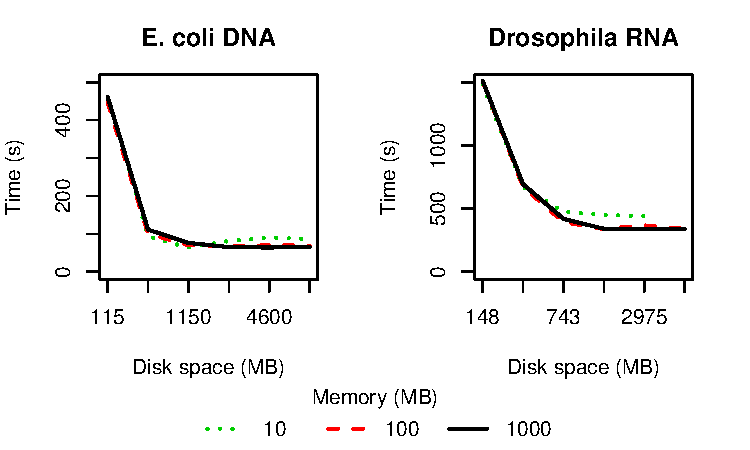
\includegraphics[width=.5\textwidth]{figure}
\caption{Execution time of \dsk ($k=21$) as a function of memory and disk usage, on the \emph{E. coli} (Illumina DNA SRR001665, $20.8\cdot 10^6$ reads of average length $36$ bp) and \emph{D. ananassae} datasets (Illumina RNA-Seq SRR332538 $9.1\cdot 10^6$ reads of average length $150$ bp).}
\end{figure}


\section{Discussion}

Contrary to other methods, \dsk does not provide random access to $k$-mer counts. However, it benefits from three strong points:
%Compared to  \jelly and \bfc 
%other methods, \dsk has three strong points:

\begin{itemize}
\item \textbf{Low memory usage}: Only an arbitrarily small subset of $k$-mers is loaded in memory at any time. In contrast, \bfc stores all the $k$-mers with count $\geq 2$ in a hash table. In principle, \jelly can use arbitrarily small hash tables, however storing the intermediate results requires a prohibitive amount of disk ($\geq 1$ TB for human genome reads using a hash table of size 5 GB).%\bfc requires an upper bound of the number of distinct $k$-mers.
\item \textbf{Parameters are automatically inferred}: the only mandatory argument is the $k$-mer length. Optionally, target memory and disk usages can be specified. \jelly and \bfc require the user to specify respectively a hash table size and an upper-bound on the number of distinct $k$-mers.
\item \textbf{Supports arbitrarily large values of $k$}: as opposed to up to $32$ for \jelly (unbounded for \bfc).
% proof: Invalid mer length '63'. It must be in [2, 31].
\end{itemize}


%%%%%%%%%%%%%%%%%%%%%%%%%%%%%%%%%%%%%%%%%%%%%%%%%%%%%%%%%%%%%%%%%%%%%%%%%%%%%%%%%%%%%
%
%     please remove the " % " symbol from \centerline{\includegraphics{fig01.eps}}
%     as it may ignore the figures.
%
%%%%%%%%%%%%%%%%%%%%%%%%%%%%%%%%%%%%%%%%%%%%%%%%%%%%%%%%%%%%%%%%%%%%%%%%%%%%%%%%%%%%%%

%\vspace{-2cm}
\section*{Acknowledgment}

\paragraph{Funding\textcolon} ANR MAPPI, ANR-10-COSI-0004


%
%\bibliographystyle{plain}
%\bibliographystyle{achemnat}
%\bibliographystyle{plainnat}
%\bibliographystyle{abbrv}
%\bibliographystyle{bioinformatics}
%
\bibliographystyle{natbib}
\bibliography{paper}


%\begin{thebibliography}{}
%\end{thebibliography}
\end{document}
